\documentclass[a4paper]{article}
\usepackage[UTF8]{ctex}
\usepackage{geometry}
\usepackage{graphicx}
\usepackage{url}
\usepackage{multirow}
\usepackage{array}
\usepackage{booktabs}
\usepackage{url}
\usepackage{enumitem}
\usepackage{graphicx}
\usepackage{float}
\usepackage{amssymb}
\usepackage{amsmath}
\usepackage{subfig}
\usepackage{longtable}
\usepackage{pifont}
\usepackage{color}

\allowdisplaybreaks

\geometry{a4paper, scale=0.78}

\usepackage{tikz}
\newcommand*{\circled}[1]{\lower.7ex\hbox{\tikz\draw (0pt, 0pt)%
    circle (.5em) node {\makebox[1em][c]{\small #1}};}}
    

% \begin{figure}[H]
%     \centering
%     \includegraphics[width=.55\textwidth]{E.png}
%     \caption{矩阵与列向量的乘法}
%     \label{fig:my_label_1}
% \end{figure}

% \left\{
% \begin{array}{ll}
%       x+2x+z=2 & \\
%       3x+8y+z=12 & \\
%       4y+z=2
% \end{array}
% \right.

% \begin{enumerate}[itemindent = 1em, itemsep = 0.4pt, parsep=0.5pt, topsep = 0.5pt]

% \end{enumerate}

%\stackrel{a}{\longrightarrow}

%\underbrace{}_{} %下括号

%\tableofcontents %目录,并且目录页不记录页码
% \tableofcontents
% \newpage
% \setcounter{page}{1} %new page
% \clearpage

\title{Generative Model}
\author{Chen Gong}
\date{25 May 2020}

\begin{document}
\maketitle
%\pagestyle{empty}
\tableofcontents
\newpage
%\pagestyle{fancy}
\setcounter{page}{1} %new page
\clearpage
\maketitle

\section{生成模型的定义}
前面所详细描述的模型以浅层的机器学习为主。本章将承上启下引出后面深度机器学习的部分。本小节,主要讲述的是什么是生成模型,它是不是只是生成样本,生成数据?它的任务是什么?精准的定义是什么?

这个问题实际上在之前的章节中有过详细的介绍。这里更进一步总结。回忆一下,之前讲过的简单的生成模型,包括高斯混合分布(GMM),GMM的主要任务是聚类,属于非监督学习;而监督学习中的生成模型,最简单的有朴素贝叶斯模型,主要任务是分类。而Logistics regression显然不是生产模型,简单的说,LR模型主要是对$P(Y=1|X)$或$P(Y=0|X)$条件概率进行建模,并不关心样本$X$是什么样。

所以,对比一下可以发现,生成模型关注点是样本分布本身,解决的问题与任务无关,对样本分布建模。比如简单学习中,先对$P(X,Y)$建模,然后求$\sum_X P(Y|X)$来计算条件概率。在无监督学习中,直接对$P(X)$建模,由于有的时候,$P(X)$非常的复杂,直接对$P(X)$建模非常的困难。这是就会引入隐变量(Latent)$Z$,对$P(X,Z)$建模,然后$P(X) = \sum_Z P(X|Z)$。

{\color{red}生成模型关注的是样本分布本身,是对样本数据本身建模,所以一定和概率分布有关,往往被称之为“概率生成模型”。}

\section{监督 vs 非监督}
监督或非监督学习,按照任务分可以将生成模型实现的功能分成以下几种,包括:{\color{red} 分类,回归,标记,降维,聚类,特征学习,密度估计,生产数据。}
\subsection{监督任务}
监督任务中可以大致分为概率模型和非概率模型两类。实际上这两个模型之间并不是非黑即白的,两者之间的界限是模糊的,本节中做一个简单的介绍。
\subsubsection{判别模型}
判别模型是对条件概率分布建模$P(Y|X)$,典型的有Logistics Regression,最大熵马尔可夫模型(MEMM),条件随机场(CRF),这个模型听名字就很条件概率。
\subsubsection{生成模型}
生成模型大致可以分成以下几类:

\textbf{1. Naive Bayes},此模型非常简单,主要是服从朴素贝叶斯假设。朴素贝叶斯假设描述的是,样本空间各维度之间相互独立,$P(X|Y)=\prod_{i=1}^p P(x_i|Y)$。

\textbf{2. Mixture Model},其中的典型代表是混合高斯模型(GMM),此模型主要是用于聚类。模型可以简要的表示为$P(X|Z)\sim$ Gaussian Distribution.

\textbf{3. Time-series Model},最基础的有隐马尔可夫模型(HMM),卡曼滤波(Kalman Filter),粒子滤波(Particle Filter)。

\textbf{4. Non-Parameteric Model},此模型最重要的特点是参数空间无限化,参数不是一个确定的值,而是一个服从分布,比如Gaussian Process(GP)模型,此模型也是Bayesian Model的一种。

\textbf{5. Mixed member Model},其代表是LDA模型。

\textbf{6. Factorial Model},包括factor analysis,概率PCA模型(P-PCA),ICA,和稀疏编码(Sparse Coding)等等。

上述的六种模型都是浅层的生成模型,什么意思呢?简单的说就是模型的结构相对固定,变换不大,模型的层数也很较少。\textbf{下面描述的是Deep生成模型},模型结构变化较大,而且层数较多。深度生成模型中,经常将神经网络和传统概率相结合。Deep之前的模型,比较固化,基本是用来解决特定的问题。

\textbf{7. Energy based model},包括前面讲到的,Boltzmann Machines,Sigmoid Belief Network,Deep Belief Network,Deep Boltzmann Machines。其主要是基于玻尔兹曼分布的,而实际上玻尔兹曼分布为$\exp\{\mathrm{E}(\theta)\}$,可以看成是熵的形式。

\textbf{8. Variational Automation Coder},变分自编码器。

\textbf{9. GAN},生成对抗神经网络。

\textbf{10. Flow-base model},基于流的模型。

\subsubsection{非概率模型}
包括PLA,Support Vector Machines(支持向量机),KNN(K近邻网络),Tree Model,神经网络(Neural Network)注意神经网络非概率模型,但是和判别模型并不是非黑即白的关系,也可以起到判别模型的作用。其大部分情况是发挥着非概率模型的作用。

\subsection{非监督任务}
非监督任务中,概率模型都是生成模型,和前文描述的监督学习中的概率模型是一样的。这章主要讲述是非概率模型。非概率模型包括,PCA(SVD分解),LSA(潜语义分析),K-means,Auto-encoder。

\subsection{小结}
本小节主要是从任务的角度介绍了一下,可以分为监督学习和非监督学习。实际上PCA推广之后就是概率PCA(P-PCA),然后进一步发展就是因子分析(FA)。K-means算法发展得到Gaussian Mixture Model(GMM)。从auto-Encoder发展得到VAE。从LSA模型发展得到PLSA,最后得到LDA模型。很多模型都是一步步发展出来的。

\section{模型表示,推断和学习}
上一小节从监督学习或者非监督学习的角度介绍了生成模型,这小节将从模型,推断和学习表示的角度分别介绍生成模型。

\subsection{模型表示}
首先从模型表示角度介绍,我们可以用“形神兼备”四个字来描述。
\subsubsection{“形”}
“形”包括以下几个方面,可以理解为生成模型的概率图表示形式:

\textbf{1. Discrete vs Continuous},从点的角度出发,也就是说节点的变量是离散随机变量还是连续随机变量。

\textbf{2. Directed Model vs Undirected Model},从有向图和无向图的角度进行分类,有向图是贝叶斯模型,无向图是马尔可夫模型,这是从边的角度进行分析。

\textbf{3. Latent Variational Model vs Fully Observed Model},区分为所有变量可完全观测或者含有部分隐变量。

\textbf{4. Shadow vs Deep},这个是根据网络的层数来确定的。

\textbf{5. Sparse vs Dense},此分类标准根据节点之间连接的权重稠密或者稀疏而定的。比如,Boltzmann Machines之间权重的连接就比HMM之间要稠密的多,最稠密的当然是完全图了。

\subsubsection{“神”}
这个从“神”的角度来分,有一点抽象,哈哈哈!主要从以下两个方面来理解。

\textbf{6. Parameteric Model vs Non-Parameteric Model},此分类描述的是参数是确定的,还是一个分布,参数不确定,比如,高斯过程就是Non-Parameteric Model,每个时刻的参数都服从不同的高斯分布。

\textbf{7. Implicit Model vs Explicit Model},Implicit Model中最典型的就是GAN。Explicit Model的特征是对$P(X)$建模,而Implicit Model不直接考虑对$P(X)$的建模,只需要可从目标分布中采样即可。比如,GAN通过从目标分布中采样,来建立一个虚拟的分布。

\subsection{推断}
推断就很简单了,基本就是从计算可行性分析,
\textbf{8. Tractable vs Intractable}。

\subsection{学习}
学习的主要可以分为:

\textbf{9. Likelihood-based Model vs Likelihood-free Model},极大似然估计求解,是使log似然达到最大之后,用求得的参数来进行采样。而Likelihood-free方法中,学习采用的方法和Likelihood无关。

\subsection{小结}
我们从模型表示,推断和学习表示的角度分别介绍生成模型,可以得到以下9种分类。

1. Discrete vs Continuous

2. Directed Model vs Undirected Model

3. Latent Variational Model vs Fully Observed Model

4. Shadow vs Deep

5. Sparse vs Dense

6. Parameteric Model vs Non-Parameteric Model

7. Implicit Model vs Explicit Model

8. Tractable vs Intractable

9. Likelihood-based Model vs Likelihood-free Model

而我们主要关注的是比较新的模型,所以重点介绍的是,1中的Discrete;2中的两个模型,Directed Model和Undirected Model;3中的Latent Variational Model;4中的Shadow vs Deep,其中深度生成模型是后面的重点;5中的Dense;6中的Parameteric Model;7中的Implicit Model(GAN)和Explicit Model;8中Tractable和Intractable都有讲到;9中的Likelihood-based Model和Likelihood-free Model都有。

\section{Maximum Likelihood}
从Likelihood-based Model和Likelihood-free Model两个方面分,是目前比较流行的一种分法。

\subsection{Likelihood-based Model}
这是显式的估计概率密度函数,也就是Explicit Model。根据其是否可计算大致可以分成两类,tractable和intractable。

其中,Fully observed的算法一定是tractable,这样的模型结构相对很简单,典型算法有Autoregression Model。而另一类则是change of variable(Flow-based model),这里做简要的说明。假如$P(X)$非常复杂,那么我们可以对一个简单的分布$P(Z)$建模,然后寻找一个$X \mapsto Z$的映射$X=g(Z)$。那么,可得$Z = g^{-1}(X)$。此模型的主要目的就是学习这个映射$g(Z)$,可以得到
\begin{equation}
    P_X(X) = P_Z(g^{-1}(X))
\end{equation}
参数计算为$\frac{\partial g^{-1}(X)}{\partial X}$。

而关于Approximate Inference,包括两种,1. MCMC,这是一种Energy Based Model,因为其是基于随机采样的。2. 为确定性的变分推断,典型的算法有VAE。

\subsection{Likelihood-free Model}
这是不显示的概率密度函数,也就是不直接对概率密度函数建模。比如说直接从样本分布中采样的GAN,通过模拟一个分布来直接进行采样,不需要通过MCMC采样。样本直接生成分布。还有直接采样的,比如Mento Calro算法,GSN等。

\subsection{小结}
我觉得主要是从函数学习方法的角度,来进行分类,也就是是否计算似然函数。个人觉得Likelihood-free Model是目前很重要的研究,以我做的科研为例,我觉得从未知分布中采样来逼近目标分布非常重要,如果给目标分布确定的形式会造成算法的局限性,所有舍弃分布的具体,使用采样来逼近非常重要,现在比较流行的有分布式强化学习中的分位点回归法。

\section{概率图 vs 神经网络}
概率图模型和神经网络之间并不是一个非黑即白的区别,它们之间有区别也有联系,但是很多部分同学都搞不清他们之间的区别。

首先我认为他们的核心区别在于,\textbf{概率图模型是$P(X)$的表示,神经网络即时一个函数逼近器,对于一个输入的$X$,得到输出的$Y$,中间的部分都是权重。}所以,他们两压根不是一个东西,概率图模式是对$P(X)$来建模,典型的概率生成模型。

概率图模型中主要讨论的是Bayesian Network,Boltzmann Machines;神经网络是广义连接主义,确定NN有CNN,RNN。在本节中,仅比较Beyesian Network和NN。

\subsection{Bayesian vs NN}
本小节将从表示,推断,学习和适合问题四个角度出发进行比较。

\subsubsection{模型表示}
Bayesian Network是从结构化,权值之间相对稀疏,而且通常层数比较浅,符合条件独立假设。\textbf{其中最重要的是Bayesian Network具有可解释性,建模的时候具有真实的物理意义。}

而NN的层数,往往会比较深,而且权值连接很稠密,没有具体的物理意义。有的小伙伴会说,NN也具有可解释性,比如神经网络类似为一个滤波器,其可以抽象出更多的高层信息。这个东西,其实只是我们一厢情愿的,这个意义并不是在建模的时候赋予的。而是我们发现了其好的效果之后,在这里强行解释,有点“马后炮”的味道。NN的可解释性,并不关键,或者说我们都不关心。

\subsection{推断}
Bayesian Network中包括精确推断和近似推断,有MCMC和变分等方法。还有极大似然估计等等。

而神经网络的推断方法就非常的简单了,输入输出即可,没有太多的研究意义。

\subsection{学习}
Bayesian Network中常见的解决方法有Log似然梯度,EM算法等。

NN中常用的方法是梯度下降,由于这个层数很多,节点很多的时候求导很不好求,于是引入了BP算法。其实BP算法是一种高效的求导方法,其实\textbf{BP算法 = 链式求导法则+动态规划}。动态规划什么意思,就是递归+缓存。

实际上,可以感觉到Bayesian Network和神经网络都不是一个level的东西。\textbf{概率图是一个模型层次的,是对数据样本的建模。而神经网络中被称之为计算图,完全就是来计算用的。}

\subsection{适合的问题}
Bayesian Network更适合解决High Level Reasoning的问题,适合于做原因推断。

而NN更适合解决Low Level Reasoning的问题,不适合做原因推断,只能由于解决弱推理问题。其更适合表示学习。

\subsection{小结}
本章的内容比较简单,基本就是从表示,推断,学习和适合问题四个角度出发进行比较概率图模型和神经网络模型。其实这两个东西都不是一个level的,主要区别是概率图模型是对样本数据的建模,而神经网络只是一个函数逼近器而已。

\section{Stochastic Back Propagation (Reparametrization Trick)}
本章主要介绍的是,神经网络用$Y=f(X;\theta)$函数逼近器,那么我们将想想神经网络和概率图模型之间有什么关系呢?能不能用NN去逼近一个概率分布$P(X)$呢?把他们两结合到一起就是随机后向传播,或者称之为重参数技巧。

\subsection{正常情况下简单举例}
假设$P(Y)$是目标分布,其中$P(Y)\sim \mathcal{N}(\mu,\sigma^2)$。我们之前是怎么采样的呢?是先从一个简单的高斯分布中进行采样$Z\sim \mathcal{N}(0,1)$,然后令$Y = \mu + \sigma Z$,就相当于一个二元一次变换。这样就可以得到采样方法:
\begin{equation}
    \left\{
\begin{array}{ll}
      z^{(i)} \sim \mathcal{N}(0,1) & \\
      y^{(i)} = \mu + \sigma z^{(i)}  & \\
\end{array}
\right.
\end{equation}
那么很自然的可以将此函数看成,{\color{red}$y=f(\mu, \sigma, z)$}。这是一个关于$z$的函数,$\mu, \sigma$假设是确定性变量,也就是当$z$确定时,函数的值是确定的。那么,算法的目标就是找到一个函数映射$z\mapsto y$,函数的参数为$\{ \mu,\sigma \}$。

假设,$J(y)$是目标函数。那么梯度求导方法为:
\begin{equation}
    \frac{\nabla J(y)}{\nabla \theta} = \frac{\nabla J(y)}{\nabla y} \frac{\nabla y}{\nabla \theta} 
\end{equation}

\subsection{条件概率密度函数}
假设目标分布为$P(Y|X)=\mathcal{N}(X;\mu,\sigma^2)$,那么,在简单高斯分布$Z \sim \mathcal{N}(0,1)$进行采样,可以得到,
\begin{equation}
    Y=\mu(X) + \sigma(X)Z
\end{equation}
实际上可以将$X$看成输入,$Z$看成是噪声,$Y$则是输出。神经网络的参数为$\theta$。那么逻辑关系为:
\begin{equation}
    Y = \mu_\theta(X) + \sigma_\theta(X)Z
\end{equation}
网络的模型如下所示:
\begin{figure}[H]
    \centering
    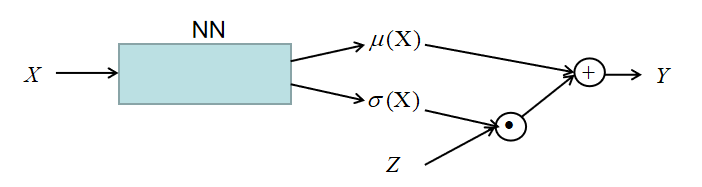
\includegraphics[width=.65\textwidth]{微信图片_20200601202036.png}
    \caption{网络逻辑关系}
    \label{fig:my_label_1}
\end{figure}
其中,$\mu(X)=f(X;\theta),\sigma(X)=f(X;\theta)$。损失函数为:
\begin{equation}
    L_\theta(Y) = \sum_{i=1}^N \|y-y^{(i)}\|^2
\end{equation}
链式求导法则为:
\begin{equation}
    \frac{\nabla J_\theta(Y)}{\nabla \theta} = \frac{\nabla J_\theta(Y)}{\nabla Y}\frac{\nabla Y}{\nabla \mu}\frac{\nabla \mu}{\nabla \theta} +
    \frac{\nabla J_\theta(Y)}{\nabla Y}\frac{\nabla Y}{\nabla \sigma}\frac{\nabla \sigma}{\nabla \theta}
\end{equation}
这样就可以做到用NN来近似概率密度函数,观测这个式子发现$Y$必须要是连续可微的,不然怎么求$\frac{\nabla Y}{\nabla \sigma}$。实际上这个模型可以被写为$P(Y|X;\theta)$,将$X,\theta$合并到一起就是$w$,所以模型也可以被写为$P(Y|w)$。

\subsection{小结}
这小结从用神经网络来近似概率分布的角度分析两种概率分布模型,简单的高斯分布和条件高斯模型。并简要的介绍了其链式求导法则。

\section{总结}
本章节主要是对于概率生成模型进行了一个全面的介绍,起到一个承上启下的作用。回顾了之前写到的浅层概率生成模型,并引出了接下来要介绍的深度概率生成模型。并从任务(监督 vs 非监督),模型表示,模型推断,模型学习四个方面对概率生成模型做了分类。并从极大似然的角度重新对模型做了分类。并介绍了概率图模型和神经网络的区别,我觉得其中最重要的是,概率图模式是对样本数据建模,其图模型有具体的意义;而神经网络只是函数逼近器,只能被称为计算图。最后,介绍了重参数技巧,用神经网络逼近概率分布,个人觉得这个思想很有意思,和我的研究内容相关,之后我会写一篇专门介绍这个。





\end{document}
